\section{CIncompatible\-Monitor  Class Reference}
\label{classCIncompatibleMonitor}\index{CIncompatibleMonitor@{CIncompatible\-Monitor}}
{\tt \#include $<$CIncompatible\-Monitor.h$>$}

Inheritance diagram for CIncompatible\-Monitor::\begin{figure}[H]
\begin{center}
\leavevmode
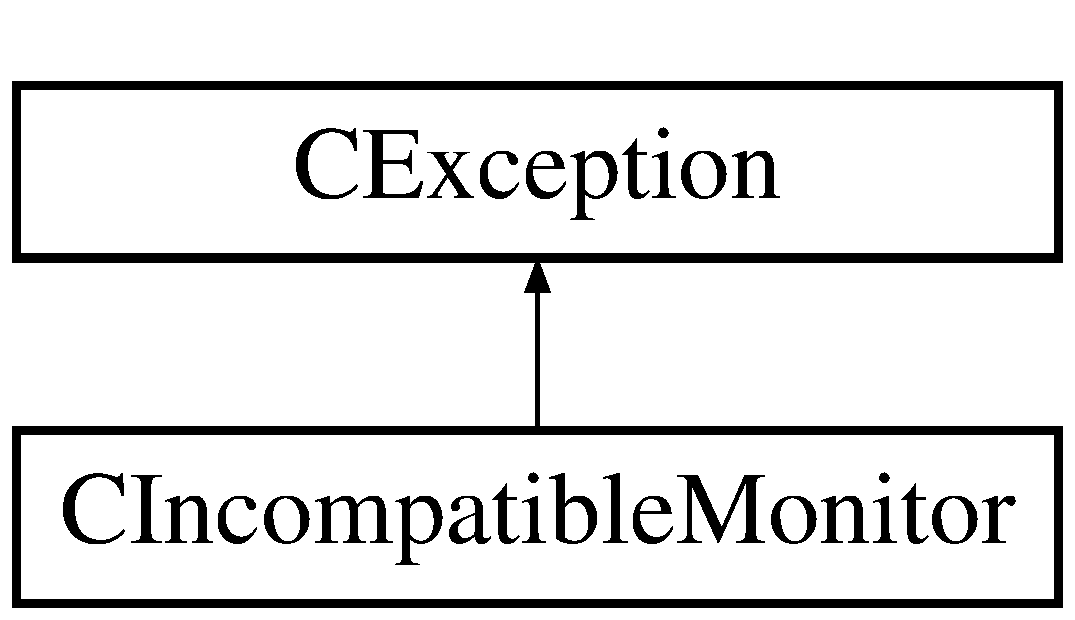
\includegraphics[height=2cm]{classCIncompatibleMonitor}
\end{center}
\end{figure}
\subsection*{Public Methods}
\begin{CompactItemize}
\item 
{\bf CIncompatible\-Monitor} ({\bf CEvent\-Monitor} \&r\-Monitor, const char $\ast$p\-Doing)
\item 
{\bf CIncompatible\-Monitor} (const CIncompatible\-Monitor \&rhs)
\item 
virtual {\bf $\sim$CIncompatible\-Monitor} ()
\item 
CIncompatible\-Monitor \& {\bf operator=} (const CIncompatible\-Monitor \&rhs)
\item 
int {\bf operator==} (const CIncompatible\-Monitor \&rhs)
\item 
string {\bf get\-Monitor\-Description} () const
\item 
void {\bf set\-Monitor\-Description} (const string \&rnew)
\item 
virtual const char $\ast$ {\bf Reason\-Text} () const
\end{CompactItemize}
\subsection*{Private Attributes}
\begin{CompactItemize}
\item 
string {\bf m\_\-Monitor\-Description}
\item 
string {\bf m\_\-Reason}
\end{CompactItemize}


\subsection{Detailed Description}
Encapsulates exceptions thrown when a reactor sense that it has been attached to an incompatible event monitor. The exception is capable of returning textual string information about the type of the monitor received and what the reactor was doing when it threw the exception. 



Definition at line 307 of file CIncompatible\-Monitor.h.

\subsection{Constructor \& Destructor Documentation}
\index{CIncompatibleMonitor@{CIncompatible\-Monitor}!CIncompatibleMonitor@{CIncompatibleMonitor}}
\index{CIncompatibleMonitor@{CIncompatibleMonitor}!CIncompatibleMonitor@{CIncompatible\-Monitor}}
\subsubsection{\setlength{\rightskip}{0pt plus 5cm}CIncompatible\-Monitor::CIncompatible\-Monitor ({\bf CEvent\-Monitor} \& {\em r\-Monitor}, const char $\ast$ {\em p\-Doing})}\label{classCIncompatibleMonitor_a0}


\char`\"{}Normal\char`\"{} Constructor. Constructs an incompatible exception object just prior to throwing it. Information from the monitor is stored as is information about what was happening in the system at the time the exception was constructed:\begin{Desc}
\item[Parameters: ]\par
\begin{description}
\item[{\em 
r\-Monitor}]- The monitor which was not compatible with the Reactor that detected the problem. \item[{\em 
p\-Doing}]- Text string describing what the program was attempting to do when the incompatibility was detected. \end{description}
\end{Desc}


Definition at line 306 of file CIncompatible\-Monitor.cpp.\index{CIncompatibleMonitor@{CIncompatible\-Monitor}!CIncompatibleMonitor@{CIncompatibleMonitor}}
\index{CIncompatibleMonitor@{CIncompatibleMonitor}!CIncompatibleMonitor@{CIncompatible\-Monitor}}
\subsubsection{\setlength{\rightskip}{0pt plus 5cm}CIncompatible\-Monitor::CIncompatible\-Monitor (const CIncompatible\-Monitor \& {\em rhs})}\label{classCIncompatibleMonitor_a1}


Copy constructor. Used by the compiler construct temporary objects or  alternatively, and more usually for this class to build a 'scope safe' copy of the exception which can be saved and passed to catch handlers. \begin{Desc}
\item[Parameters: ]\par
\begin{description}
\item[{\em 
rhs}]- the reference object being copy constructed. \end{description}
\end{Desc}


Definition at line 320 of file CIncompatible\-Monitor.cpp.\index{CIncompatibleMonitor@{CIncompatible\-Monitor}!~CIncompatibleMonitor@{$\sim$CIncompatibleMonitor}}
\index{~CIncompatibleMonitor@{$\sim$CIncompatibleMonitor}!CIncompatibleMonitor@{CIncompatible\-Monitor}}
\subsubsection{\setlength{\rightskip}{0pt plus 5cm}virtual CIncompatible\-Monitor::$\sim$CIncompatible\-Monitor ()\hspace{0.3cm}{\tt  [inline, virtual]}}\label{classCIncompatibleMonitor_a2}




Definition at line 318 of file CIncompatible\-Monitor.h.

\subsection{Member Function Documentation}
\index{CIncompatibleMonitor@{CIncompatible\-Monitor}!getMonitorDescription@{getMonitorDescription}}
\index{getMonitorDescription@{getMonitorDescription}!CIncompatibleMonitor@{CIncompatible\-Monitor}}
\subsubsection{\setlength{\rightskip}{0pt plus 5cm}string CIncompatible\-Monitor::get\-Monitor\-Description () const\hspace{0.3cm}{\tt  [inline]}}\label{classCIncompatibleMonitor_a5}




Definition at line 325 of file CIncompatible\-Monitor.h.

References m\_\-Monitor\-Description.\index{CIncompatibleMonitor@{CIncompatible\-Monitor}!operator=@{operator=}}
\index{operator=@{operator=}!CIncompatibleMonitor@{CIncompatible\-Monitor}}
\subsubsection{\setlength{\rightskip}{0pt plus 5cm}CIncompatible\-Monitor \& CIncompatible\-Monitor::operator= (const CIncompatible\-Monitor \& {\em rhs})}\label{classCIncompatibleMonitor_a3}


Assignment operator. .much like copy construction except:\begin{CompactItemize}
\item 
We gaurd against self assignment problems.\item 
We are already a fully constructed object in our own right.\item 
We return a refereince to $\ast$this.\end{CompactItemize}
\begin{Desc}
\item[Parameters: ]\par
\begin{description}
\item[{\em 
rhs}]- the object being assigned to us. \end{description}
\end{Desc}


Definition at line 335 of file CIncompatible\-Monitor.cpp.

References m\_\-Monitor\-Description, and CException::operator=().\index{CIncompatibleMonitor@{CIncompatible\-Monitor}!operator==@{operator==}}
\index{operator==@{operator==}!CIncompatibleMonitor@{CIncompatible\-Monitor}}
\subsubsection{\setlength{\rightskip}{0pt plus 5cm}int CIncompatible\-Monitor::operator== (const CIncompatible\-Monitor \& {\em rhs})}\label{classCIncompatibleMonitor_a4}


Equality comparison. We do base class comparison and compare the monitor description. The m\_\-Reason string is not relevant.\begin{Desc}
\item[Parameters: ]\par
\begin{description}
\item[{\em 
rhs}]- Reference to object we compare ourselves to. \end{description}
\end{Desc}


Definition at line 351 of file CIncompatible\-Monitor.cpp.

References m\_\-Monitor\-Description, and CException::operator==().\index{CIncompatibleMonitor@{CIncompatible\-Monitor}!ReasonText@{ReasonText}}
\index{ReasonText@{ReasonText}!CIncompatibleMonitor@{CIncompatible\-Monitor}}
\subsubsection{\setlength{\rightskip}{0pt plus 5cm}const char $\ast$ CIncompatible\-Monitor::Reason\-Text () const\hspace{0.3cm}{\tt  [virtual]}}\label{classCIncompatibleMonitor_a7}


Returns a description of why the exception is being thrown. This is of the form: Incompatible Event monitor found: \char`\"{}monitor description\char`\"{}, while: Doing\char`\"{} 

Reimplemented from {\bf CException} {\rm (p.\,\pageref{classCException_a8})}.

Definition at line 363 of file CIncompatible\-Monitor.cpp.

References m\_\-Monitor\-Description, m\_\-Reason, and CException::Was\-Doing().\index{CIncompatibleMonitor@{CIncompatible\-Monitor}!setMonitorDescription@{setMonitorDescription}}
\index{setMonitorDescription@{setMonitorDescription}!CIncompatibleMonitor@{CIncompatible\-Monitor}}
\subsubsection{\setlength{\rightskip}{0pt plus 5cm}void CIncompatible\-Monitor::set\-Monitor\-Description (const string \& {\em rnew})\hspace{0.3cm}{\tt  [inline]}}\label{classCIncompatibleMonitor_a6}




Definition at line 331 of file CIncompatible\-Monitor.h.

References m\_\-Monitor\-Description.

\subsection{Member Data Documentation}
\index{CIncompatibleMonitor@{CIncompatible\-Monitor}!m_MonitorDescription@{m\_\-MonitorDescription}}
\index{m_MonitorDescription@{m\_\-MonitorDescription}!CIncompatibleMonitor@{CIncompatible\-Monitor}}
\subsubsection{\setlength{\rightskip}{0pt plus 5cm}string CIncompatible\-Monitor::m\_\-Monitor\-Description\hspace{0.3cm}{\tt  [private]}}\label{classCIncompatibleMonitor_o0}




Definition at line 311 of file CIncompatible\-Monitor.h.

Referenced by get\-Monitor\-Description(), operator=(), operator==(), Reason\-Text(), and set\-Monitor\-Description().\index{CIncompatibleMonitor@{CIncompatible\-Monitor}!m_Reason@{m\_\-Reason}}
\index{m_Reason@{m\_\-Reason}!CIncompatibleMonitor@{CIncompatible\-Monitor}}
\subsubsection{\setlength{\rightskip}{0pt plus 5cm}string CIncompatible\-Monitor::m\_\-Reason\hspace{0.3cm}{\tt  [private]}}\label{classCIncompatibleMonitor_o1}




Definition at line 312 of file CIncompatible\-Monitor.h.

Referenced by Reason\-Text().

The documentation for this class was generated from the following files:\begin{CompactItemize}
\item 
{\bf CIncompatible\-Monitor.h}\item 
{\bf CIncompatible\-Monitor.cpp}\end{CompactItemize}
